\documentclass[conference]{IEEEtran}

\usepackage{graphicx}
\usepackage[super]{nth}

\begin{document}
	
	\title{Chinese Borders}
	
	\author{\IEEEauthorblockN{Ida Hönigmann}
		\IEEEauthorblockA{Technical Secondary College\\
			Department of Computer Science\\
			2700 Wiener Neustadt, Austria\\
			Email: hoenigmann.ida@student.htlwrn.ac.at}
	}
	
	\maketitle
	
	\begin{abstract}
		The abstract goes here.
	\end{abstract}
	
	\section{Introduction}
	As China is not particularly friendly to most of its neighbouring countries and has the longest land border in the world, it is no wonder that there are several disputes and even more interesting facts about these lines on the map.
	
	The topic of Chinese borders gives an insight into Chinese history, for which the Russian and Mongolian relations to China as well as Hong Kong and Macau are examples. It explores who and what gets transported out and into the country, such as workers building the Belt and Road Initiative, products being sold by China and North Koreans fleeing their country. Border disputes and the people living in these regions are yet another interesting case study along the Chinese border to Pakistan, India, Bhutan, Myanmar and, although already resolved, Nepal. While one would think being a communist lead country would help increase the relation to China, as it did with Laos, Vietnam shows that China is more picky and looks for more than just political beliefs. After having established all these interesting relations to all of its bordering countries China on land it tried extending its influence on the South China Sea. 
	
	\section{North Korea}
	Along the border separating China from North Korea lies one of the holy sights of all Koreans: Mount Paektu. \cite{theIndianExpress_explainedWhatIsTheSignificanceOfMtPeaktuForKinJongUn} Here South Koreans as well as North Koreans visit the Heaven Lake, although separated by multiple meters, as to not be able to see one another. From this mountain the two rivers Yalu and Tumen form. These rivers serve as the separation between the two countries.
	
	Further west in Dandong a significant portion of North Korea's trade with the outside world is being moved by trucks over a single bridge. These trucks are being loaded up in China and send to North Korea, where they are unloaded and send back - mostly empty. The imports from China make up about 57\%\cite{wp_economyOfNorthKorea} of Norths Korea's imports in total.
	
	One of the reasons China is exporting so many goods to North Korea is fear of the regime collapse, which would send thousands of North Korean emigrants over the border to China.
	
	As there are already some defectors crossing the border further east, the shallow river is protected by Chinese guards.\cite{yp_anInconvenientBorderWhereChinaMeetsNorthKoreaABCNews} All fleeing persons found, are send back to North Korea, where they will most likely face death.
	
	\section{India and Pakistan}
	The border shared with India is crowded with border disputes. The rough terrain made it impossible to establish borders for the longest time in history. Now, with the technology to reach these isolated sections, many nations claim their chunk.
	
	\subsection{Jammu and Kashmir}
	When Britain left India they decided to split the country into a Moslem (now called Pakistan and Bangladesh) and a Hindu (still called India) part, according to the affiliation of people living in each region. In some regions the local ruler could choose to which side the region should belong. In Jammu and Kashmir the ruler opted for independence of both, but after being invaded by Pakistan, turned to India.
	
	The northern part of Jammu and Kashmir, Aksai Chin, is hard to access from India. So when China built a road through this terrain during the 1950s, India did not notice until 1957. Since then Aksai Chin in administered by China. A section of the road can be seen in figure~\ref{pic:india_jammuAndKashmir_road}.
	
	\begin{figure}[t]
	\centering
	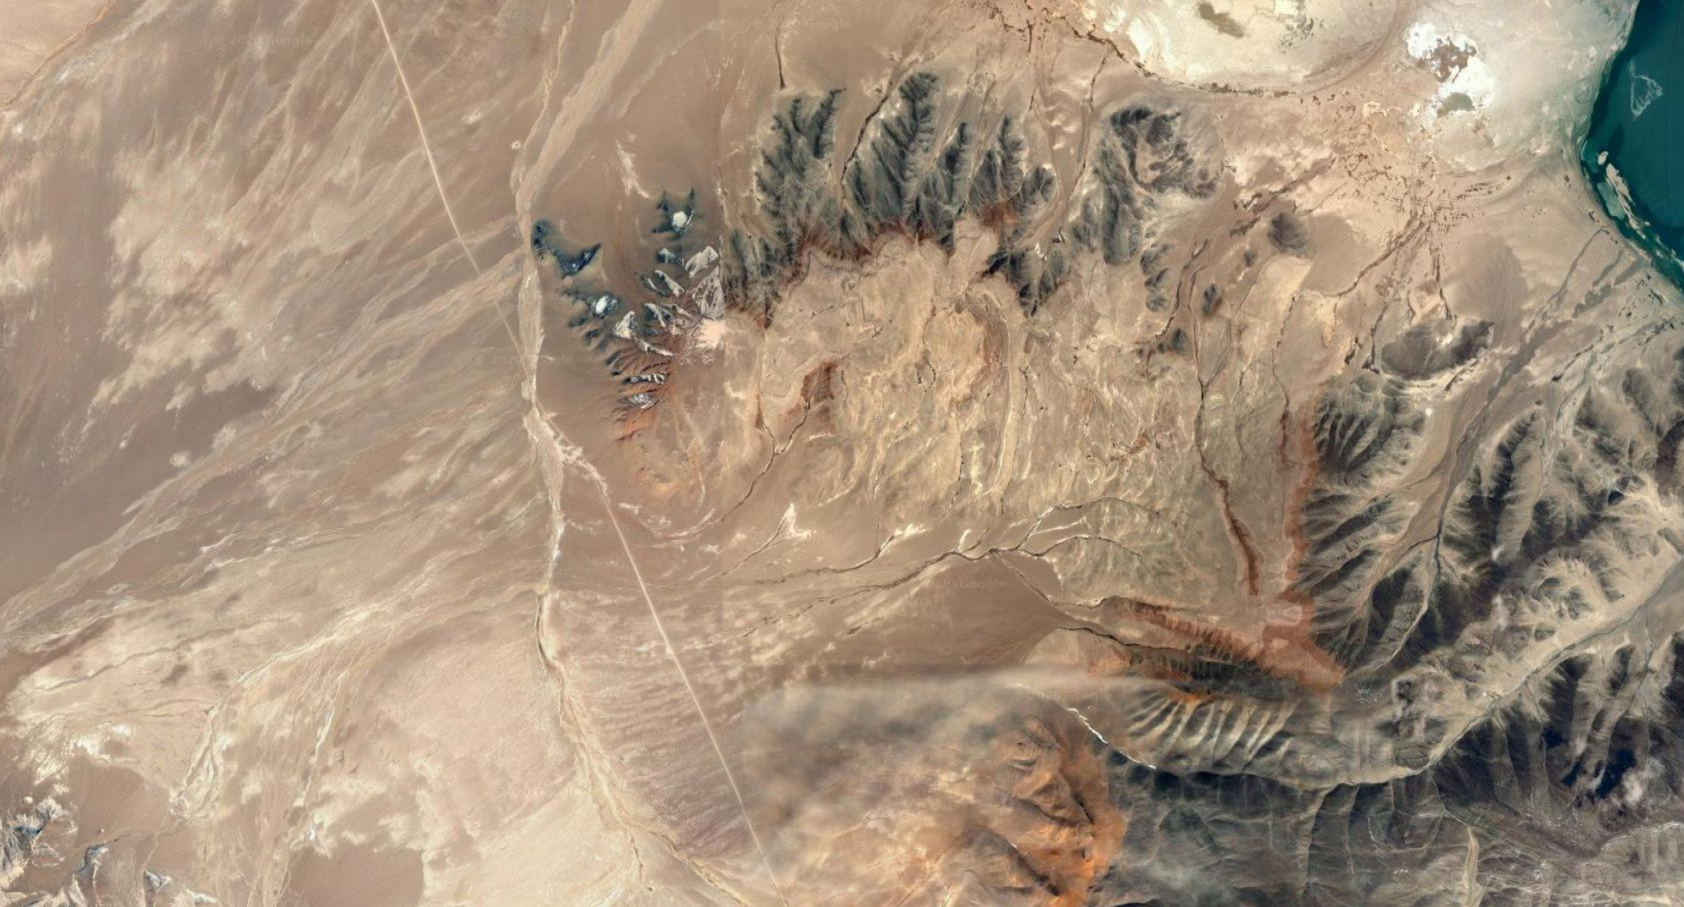
\includegraphics[width=\linewidth]{img/india_jammuAndKashmir_road.png}
	\caption{Satellite image of a part of Aksai Chin from Google Maps. The road goes from the top left to the bottom centre of the image and has a light brown colour.}
	\label{pic:india_jammuAndKashmir_road}
	\end{figure}
	
	\subsection{Arunachal Pradesh}
	Arunachal Pradesh is a region located between China and India both regionally and culturally. While it is governed by India the native spoken language in this region is Tibetan. Therefore China claims the region it refers to as South Tibet.
	
	\section{Hong Kong and Macau}
	The border between Hong Kong and China divides not countries, but values. Both Hong Kong and Macau were foreign colonies and are therefore what is called a special administrative region, which means they are allowed to have their own laws.
	
	One of the most obvious differences between mainland China and Macau it the absence of the law that forbids gambling. This has transformed Macaus skyline into string of casinos. In 2018 the World Bank estimated Macaus GDP to be around 54 billion US dollars.
	
	Hong Kong on the other hand is known for its freedom of speech, which has led many people reporting on the Chinese regime to move to this island. China, however, is starting to intervene in the high valued right of freedom. The protest from the Hong Kong citizens against this behaviour was called umbrella movement.
	
	Both borders are separating China from what is technically also China. The procedure of crossing is very similar to an international border, as you need your passport and a visa for China\cite{macauLifestyle_macauZhuhaiTheUltimateBorderCrossingGuide} \cite{yp_chinaIsErasingItsBorderWithHongKong}.
	
	\section{South China Sea}
	The Spratly Islands, located in the South China Sea, near the shore of the Philippines, are the objective of a relatively new extension of Chinas borders. Since 2014 seven of the reefs located there have had huge amounts of sand heaped on them. Now the newly formed islands serve military purposes, as can be seen in figure~\ref{pic:southChinaSea_subiReef}. By owning these islands China would increase exclusive economic zone, defined by the United Nations Convention on the Law of the Sea\cite{unitedNations_lawOfTheSea}.
	
	\begin{figure}[t]
		\centering
		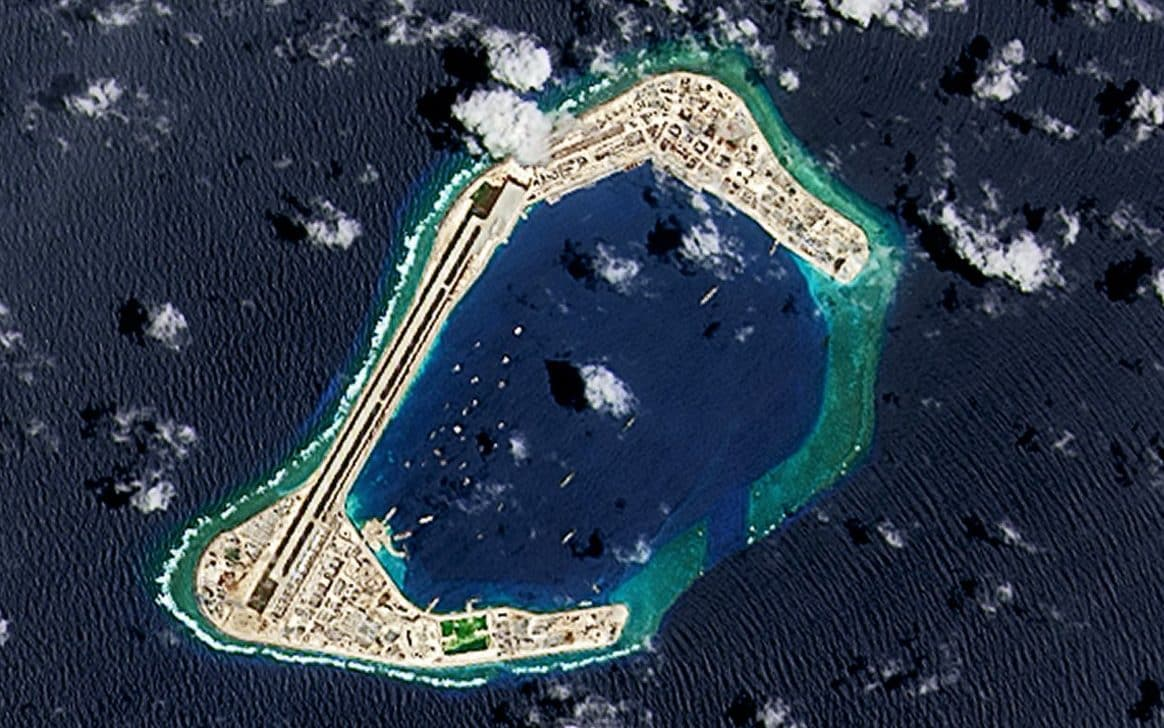
\includegraphics[width=\linewidth]{img/southChinaSea_subiReef.jpg}
		\caption{Satellite image of Subi Reef\cite{theTelegraph_chinaLandsMilitaryPlaneAtThirdSpratlyIsland}. The runway and some boats are clearly visible.}
		\label{pic:southChinaSea_subiReef}
	\end{figure}
	
	\section{Mongolia}
	Next to Mongolia lies the Chinese province of Inner Mongolia. In this province the Great Wall of China protected Chinese citizens from Mongols in the \nth{5} century BC up until the \nth{17} century AD\cite{worldAtlas_whyWasTheGreatWallOfChinaBuilt}. As the map of the Great Wall of China shows, rather than building a single line where the border is, the wall was constructed over a long period of time and moved regularly. This can be seen in figure~\ref{pic:mongolia_greatWallOfChina}.
	
	\begin{figure}[t]
		\centering
		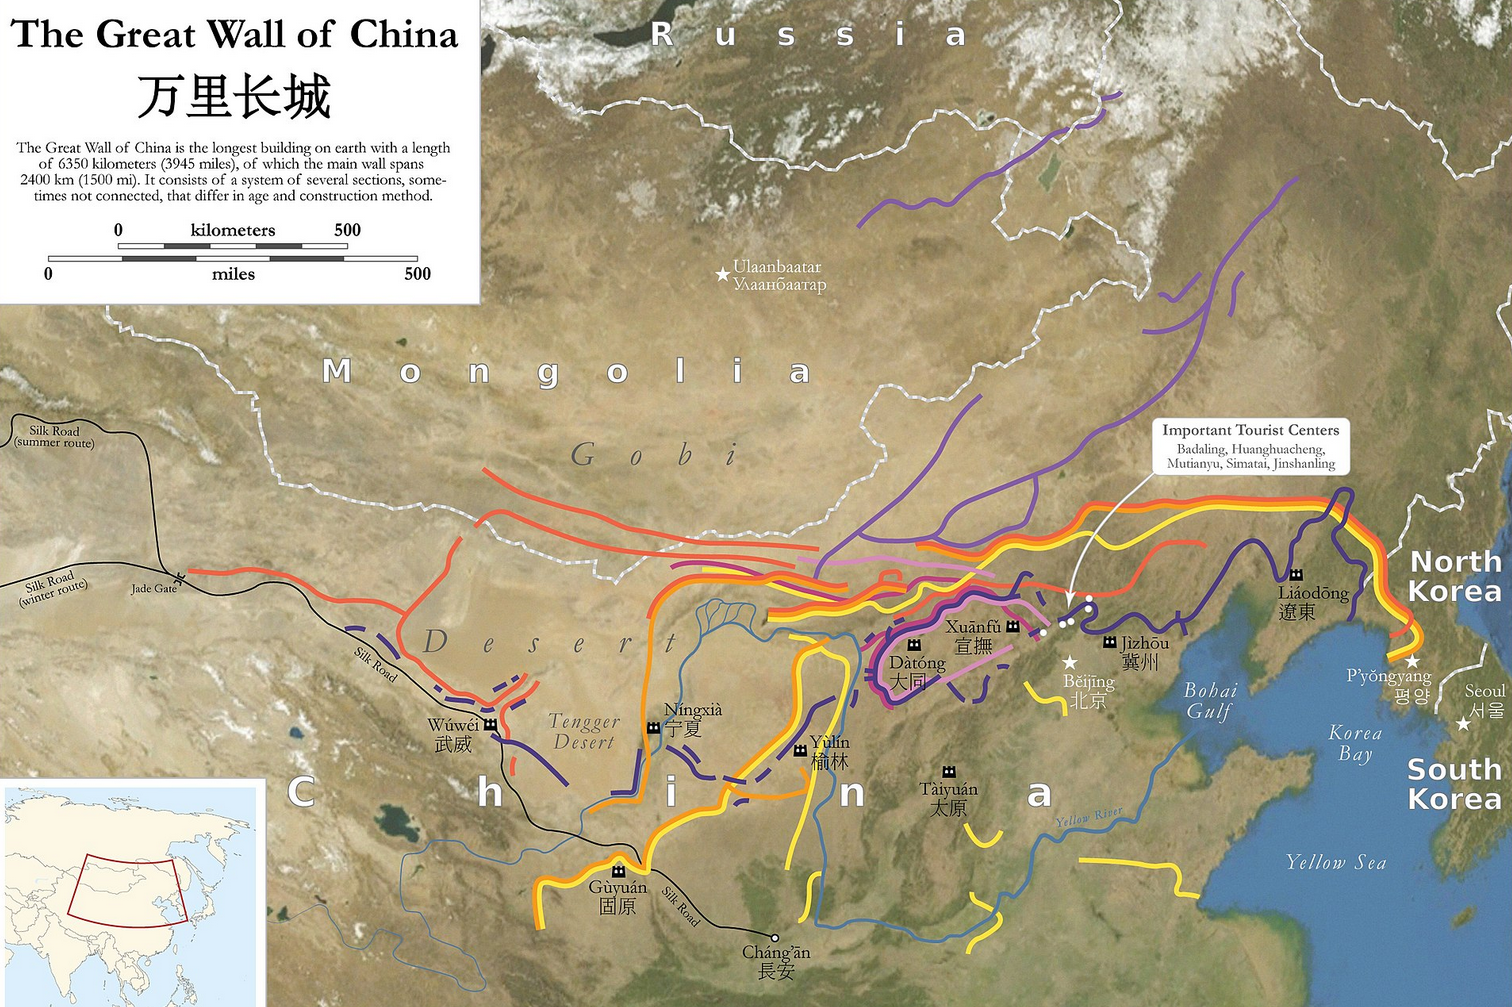
\includegraphics[width=\linewidth]{img/mongolia_greatWallOfChina.png}
		\caption{A section of the map published by Wikipedia\cite{wp_greatWallOfChina}. The different colours represent different ages in which the sections where constructed. The light purple lines represent wall segments from the \nth{11} and \nth{12} century AD and extend north into nowadays Mongolia and Russia.}
		\label{pic:mongolia_greatWallOfChina}
	\end{figure}

	Since then the Mongol Empire has collapsed. Now most people with a Mongol ethnicity live in Inner Mongolia (about 50\% more than in the state Mongolia).
	
	The Trans-Siberian Railway partly running through Mongolia transports travellers and freight between Russia and China. Now this railway network is becoming part of Chinas Belt and Road Initiative.
	
	\section{Russia}
	
	\section{Kazakhstan}
	
	\section{Kyrgyzstan}
	
	\section{Tajikistan}
	
	\section{Afghanistan}
	
	\section{Nepal}
	
	\section{Bangladesh}
	
	\section{Bhutan}
	
	\section{Myanmar}
	
	\section{Laos}
	
	\section{Vietnam}
	
	\section{Conclusion}
	The conclusion goes here.
	
	\section*{Acknowledgment}
	The authors would like to thank...
	
	\bibliographystyle{plain}
	\bibliography{main}
\end{document}


